\chapter{Função definida por partes}

\begin{obs}
Uma função $f: A \to \R$, para $A \subset \R$, é dita ser definida por partes, quando particionamos o domínio $A$ em subconjuntos disjuntos $U_i$ tais que $A= \bigcup_{i}U_i$, e para cada $U_i$ a função é dada por uma regra diferente. 
\end{obs}

\begin{exem}
\begin{equation*}
f(x) = \begin{cases}
                 3x + 4, \text{ se } x < 2 \\
                 7 , \text{ se } x = 2 \\
                 -x^2 + 8, \text{ se } x > 2
                \end{cases} \ .
\end{equation*}
   \begin{figure}[H]
  \centering
  \fbox{\includegraphics[width=7cm,height=6cm]{./cap_funcao/figs/funcaoPartesexem1}}
   \caption{Gráfico da função $f$}
  \end{figure}
\end{exem}

\begin{exem}
\begin{equation*}
f(x) = \begin{cases}
                 -x^2 + 1, \text{ se } x < 0 \\
                 e^x, \text{ se } x \geqslant 0
                \end{cases} \ .
\end{equation*}
   \begin{figure}[H]
  \centering
  \fbox{\includegraphics[height=6cm]{./cap_funcao/figs/funcaoPartesexem2}}
   \caption{Gráfico da função $f$}
  \end{figure}
\end{exem}

\begin{exem}
\begin{equation*}
f(x) = \begin{cases}
                 -x + 1, \text{ se } x \leqslant 1 \\
                 ln(x), \text{ se } x > 1
                \end{cases} \ .
\end{equation*}
\begin{figure}[H]
  \centering
  \fbox{\includegraphics[height=6cm]{./cap_funcao/figs/funcaoPartesexem3}}
   \caption{Gráfico da função $f$}
  \end{figure}
\end{exem}

\begin{exem}
\begin{equation*}
f(x) = \begin{cases}
                 x^2+2x+1, \text{ se } x < 1 \\
                 5, \text{ se } x = 1 \\
                -x+5, \text{ se } x > 1
                \end{cases} \ .
\end{equation*}
\begin{figure}[H]
  \centering
  \fbox{\includegraphics[height=7cm]{./cap_funcao/figs/funcaoPartesexem4}}
   \caption{Gráfico da função $f$}
  \end{figure}
\end{exem}

\section{Função modular}

  Considere a função $f: \R \rightarrow \R$, dada por $f(x)= \abs{x}$. Pela definição de módulo, temos que $f$ é uma função definida por partes, da seguinte forma:

  \[f(x)= \abs{x} = \begin{cases}
                 x, \text{ se } x \geq 0 \\
                 -x, \text{ se } x < 0.
                \end{cases}\]

O gráfico desta função é dada por

  \begin{figure}[H]
 \centering
    \fbox{\includegraphics[width=7cm]{./cap_funcao/figs/funcaomodulo}}
    \caption{Gráfico da função módulo}
  \end{figure}

Note que, $Im(f)= [0, \infty)$ e não todo o contradomínio $\R$. Além disso, esta é uma função na qual as duas partes são lineares.
  
 \begin{exem}
 Vamos determinar os intervalos de crescimento e decrescimento, caso existam, da função $f(x)= \abs{x}$. Lembramos que esta função é definida por partes, por isso faremos a análise em cada uma destas partes.

  Caso 1: Se $x < 0$, temos que $f(x)= -x$, logo se $x_1 < x_2$,
\begin{equation*}
x_1 < x_2 \Rightarrow -x_1 > -x_2 \Rightarrow f(x_1) > f(x_2) \ ,
\end{equation*}
  por exemplo, sendo $x_1= -3$ e $x_2= -2$ temos que $x_1 < x_2$,
\begin{equation*}
f(x_1)= f(-3)= -(-3)= 3 > 2= -(-2)= f(-2)= f(x_2) \ .
\end{equation*}

  Portanto se $x < 0$ temos que $f$ é decrescente.

  Caso 2: Se $x \geq 0$, temos que $f(x)= x$, logo se $x_1 < x_2$
\begin{equation*}
x_1 < x_2 \Rightarrow  f(x_1) < f(x_2) \ ,
\end{equation*}
  por exemplo, sendo $x_1= 2$ e $x_2= 3$ temos que $x_1 < x_2$,
\begin{equation*}
f(x_1)= 2 > 3= f(x_2) \ .
\end{equation*}

  Portanto se $x \geq 0$ temos que $f$ é crescente.
 \end{exem}

\begin{exem}
  Consideramos a função $f: \R \rightarrow \R$ dada por $f(x)= \abs{x-2}$. A função $f$ pode ser escrita como:
    \begin{align*}
        f(x)& = 
        \begin{cases}
         x -2, \text{ se } x-2 \geq 0 \\
         -(x - 2), \text{ se } x-2 < 0
        \end{cases} \\
        & = 
        \begin{cases}
         x -2, \text{ se } x \geq 2 \\
         -x +2, \text{ se } x < 2.
        \end{cases}
    \end{align*}
  Com isso a função modular pode ser vista como uma função linear por partes cujo gráfico é dado por:
  \begin{center}
  \begin{tikzpicture}[scale=1]
    \tkzInit[xmin=-1, xmax=5, xstep=1, ymin=-1,ymax=3]
        %\tkzDrawXY
        \tkzAxeXY[fill=black!5]
        
        \tkzFct[thick,red,domain=2:5]{x-2}
        \tkzFct[thick,red,domain=-4:2]{-x+2}
    
        %\tkzDefPointByFct[ref=A, with=a](-1)
        %\tkzDefPoint(0,2){A}
        %\tkzDefPoint(0.5,2.25){B}
        %\tkzPointShowCoord(B)
        %\tkzDrawPoint[fill=red, size=3](A)
        %\tkzDrawPoint[fill=red, size=3](B)
        
    \end{tikzpicture}
\end{center}
\end{exem}

\begin{exem}
  Consideramos a função $f: \R \rightarrow \R$ dada por $f(x)= \abs{x+1}+2$. A função $f$ pode ser escrita como:
    \begin{align*}
        f(x)& = 
        \begin{cases}
         x +1 +2, \text{ se } x+1 \geq 0 \\
         -(x +1) +2, \text{ se } x+1 < 0
        \end{cases} \\
        & = 
        \begin{cases}
         x +3, \text{ se } x \geq 1 \\
         -x +1, \text{ se } x < -1.
        \end{cases}
    \end{align*}
  Com isso a função modular pode ser vista como uma função linear por partes cujo gráfico é dado por:
  \begin{center}
  \begin{tikzpicture}[scale=1]
    \tkzInit[xmin=-3, xmax=3, xstep=1, ymin=0,ymax=4]
        %\tkzDrawXY
        \tkzAxeXY[fill=black!5]
        
        \tkzFct[thick,red,domain=-1:3]{x+3}
        \tkzFct[thick,red,domain=-3:-1]{-x+1}
    
        %\tkzDefPointByFct[ref=A, with=a](-1)
        %\tkzDefPoint(0,2){A}
        %\tkzDefPoint(0.5,2.25){B}
        \tkzPointShowCoord((-1,2))
        %\tkzDrawPoint[fill=red, size=3](A)
        %\tkzDrawPoint[fill=red, size=3](B)
        
    \end{tikzpicture}
\end{center}
\end{exem}

\begin{exem}
  Seja $f: \R \rightarrow \R$ dada por $f(x)= \abs{x^2-3x+2}$.
  A função $f$ pode ser escrita como:
    \begin{align*}
        f(x)& = 
        \begin{cases}
         x^2-3x+2, \text{ se } x^2-3x+2 \geq 0 \\
         -(x^2-3x+2), \text{ se } x^2-3x+2 < 0.
        \end{cases}
    \end{align*}
  A maneira mais fácil de se obter o gráfico é desenhar o gráfico da função quadrática $g(x)=x^2-3x+2$ e em seguida refletir em relação ao eixo $x$ a parte do gráfico que está abaixo deste eixo $x$, como a seguir:
  \begin{center}
  \begin{tikzpicture}[scale=1]
    \tkzInit[xmin=-1, xmax=4, xstep=1, ymin=-1,ymax=4]
        %\tkzDrawXY
        \tkzAxeXY[fill=black!5]
        
        \tkzFct[thick,red,domain=-1:1]{x**2-3*x+2}
        \tkzFct[thick,red,domain=2:4]{x**2-3*x+2}
        \tkzFct[thick,red,domain=1:2]{-x**2+3*x-2}
        \tkzFct[dashed,gray,domain=1:2]{x**2-3*x+2}

        \tkzDefPoint(1.5,0.25){A}
        %\tkzDefPointByFct[ref=A, with=a](-1)
        %\tkzDefPoint(0,2){A}
        %\tkzDefPoint(0.5,2.25){B}
        \tkzPointShowCoord[xlabel=$\frac{3}{2}$]((1.5,0.25))
        %\tkzDrawPoint[fill=red, size=3](A)
        %\tkzDrawPoint[fill=red, size=3](B)
        
    \end{tikzpicture}
\end{center}
\end{exem}

\begin{exem}
  Seja $f: \R \rightarrow \R$ dada por $f(x)= \abs{2x-4}+\abs{x-1}$. Para remover os módulos desta função consideremos as funções $f_1(x)=\abs{2x-4}$ e $f_2(x)=\abs{x-1}$. Assim,
    \begin{align*}
        f_1(x)& = 
        \begin{cases}
         2x-4, \text{ se } 2x-4 \geq 0 \\
         -(2x-4), \text{ se } 2x-4 < 0.
        \end{cases}= 
        \begin{cases}
         2x-4, \text{ se } x \geq 2 \\
         -2x+4, \text{ se } x < 2,
        \end{cases} \\
        f_2(x)& = 
        \begin{cases}
         x-1, \text{ se } x-1 \geq 0 \\
         -(x-1), \text{ se } x-1 < 0.
        \end{cases}= 
        \begin{cases}
         x-1, \text{ se } x \geq 1 \\
         x-1, \text{ se } x < 1.
        \end{cases} \\
    \end{align*}

    Somando $f_1$ com $f_2$ conforme a tabela obtemos:   
    \begin{center}
    \begin{tabular}{cccc}
        %\toprule
        & $x<1$ & $1\leq x <2$  & $x \geq 2$  \\ \midrule
        $f_1(x)=|2x-4|$ & $-2x+4$ & $-2x+4$ & $2x-4$ \\ \midrule
        $f_2(x)=\abs{x-1}$ & $-x+1$ & $x-1$ & $x-1$\\ \midrule
        $f(x)=\abs{2x-4}+\abs{x-1}$ & $-3x+5$ & $-x+3$ & $3x-5$ \\
        %\bottomrule
    \end{tabular}
    \end{center}

    Ou seja, temos que
    \begin{align*}
        f(x)& = 
        \begin{cases}
         -3x+5, \text{ se } x < 1 \\
         -x+3, \text{ se } 1\leq x<2 \\
         3x-5, \text{ se } x\geq 2.
        \end{cases}
    \end{align*}
    
    Assim, o gráfico de $f$ é dado a seguir:  
  \begin{center}
  \begin{tikzpicture}[scale=1]
    \tkzInit[xmin=0, xmax=4, xstep=1, ymin=0,ymax=5]
        %\tkzDrawXY
        \tkzAxeXY[fill=black!5]
        
        \tkzFct[thick,red,domain=-1:1]{-3*x+5}
        \tkzFct[thick,red,domain=1:2]{-x+3}
        \tkzFct[thick,red,domain=2:4]{3*x-5}

        %\tkzDefPoint(1.5,0.25){A}
        %\tkzDefPointByFct[ref=A, with=a](-1)
        %\tkzDefPoint(0,2){A}
        %\tkzDefPoint(0.5,2.25){B}
        %\tkzPointShowCoord[xlabel=$\frac{3}{2}$]((1.5,0.25))
        %\tkzDrawPoint[fill=red, size=3](A)
        %\tkzDrawPoint[fill=red, size=3](B)
        
    \end{tikzpicture}
\end{center}
\end{exem}

\begin{secExercicios}
    \begin{exer}
        Dadas as funções $f:\R\to\R$ definidas a seguir, construa seus gráficos e determine sua imagem:
        \begin{enumerate}[a)]
            \item $f(x) = 
            \left\{\begin{array}{cl}
             -x-1 & \text{ se } x \leq -2 \\
             1 & \text{ se } -2< x \leq 0 \\
             x+1 & \text{ se } x>0
            \end{array}\right.$

            \item $f(x) = 
            \left\{\begin{array}{cl}
             x+3, \text{ se } x <-1 \\
             2, \text{ se } -1 \leq x \leq 1 \\
             -x, \text{ se } x>1
            \end{array}\right.$
            
            \item $f(x) = 
            \left\{\begin{array}{cl}
             -3, \text{ se } x < -2 \\
             -x-2, \text{ se } -2\leq x\leq 0 \\
             x^2, \text{ se } x>0
            \end{array}\right.$
            
            \item $f(x) = 
            \left\{\begin{array}{cl}
             -\abs{x}, \text{ se } x < -3 \\
             -2, \text{ se } -3\leq x\leq 0 \\
             x-2, \text{ se } x>0
            \end{array}\right.$

            \item $f(x) = 
            \left\{\begin{array}{cl}
             x^2-2x-8, \text{ se } x \leq 2 \text{ ou } x\geq 4 \\
             -x^2+2x+8, \text{ se } -3< x < 4
            \end{array}\right.$
        \end{enumerate}
    \end{exer}

    \begin{exer}
        Determine o gráfico e a imagem de cada uma das funções $f:\R\to\R$ a seguir:
        \begin{enumerate}[a)]
            \item $f(x)=\abs{2x+5}$
            \item $f(x)=\abs{-3x+\frac{5}{2}}$
            \item $f(x)=\abs{-x^2-x+6}$
            \item $f(x)=\abs{2x+6}-4$
            \item $f(x)=\abs{x^2-2x-2}+5$
            \item $f(x)=\abs{x}+x$
            \item $f(x)=\abs{3x-6}+x-1$
            \item $f(x)=\abs{2x^2+3x-2}+3x+2$
            \item $f(x)=\abs{4x+4}-\abs{3x-4}$
            \item $f(x)=\abs{\abs{3x+2}-3}$
            \item $f(x)=\abs{\abs{x^2-4}-6}$
        \end{enumerate}
    \end{exer}

    \begin{exer}
        Esboce o gráfico da função $f:[-1,1]\to\R$ dada por $f(x)=x+\dfrac{\abs{x}}{x}$.
    \end{exer}

    \begin{exer}
        Determine o maior domínio da função real $f$ definida por $f(x)=\dfrac{\sqrt{\abs{x}}}{x}$.
    \end{exer}

    \begin{exer}
        (UERJ) O volume de água em um tanque varia com o tempo de acordo com a seguinte equação:
        $$
        V= 10-\abs{4-2t}-\abs{2t-6}, \text{ com } t\geq 0.
        $$
        Nela, $V$ é o volume medido em $m^3$ após $t$ horas, contadas a partir de 8h da uma manhã. Determine os horários inicial e final dessa manhã em que o volume permanece constante.
    \end{exer}
    
\end{secExercicios}